

\begin{center}
\Huge
Forberedelse til prøve	
\end{center}

\subsection*{Opgave 1 (Uden hjælpemidler)}

\begin{enumerate}[label=\roman*)]
	\item Bestem fremskrivningsfaktoren og begyndelsesværdien for eksponentialfunktionen $f$ givet ved
	\begin{align*}
		f(x) = 7\cdot 1.3^x
	\end{align*}
	\item Bestem vækstraten for eksponentialfunktionen $g$ givet ved
	\begin{align*}
		g(x) = 0.7\cdot 0.9^x
	\end{align*}
	og beskriv, hvad denne fortæller om væksten for $g$. 
\end{enumerate}


\subsection*{Opgave 2 (Med hjælpemidler)}

I en by er der i år 2000 $750\TS 000$ personer. Antallet af personer stiger med 3$\%$ om året.
\begin{enumerate}[label = \roman*)]
	\item Opskriv en model, der beskriver antallet af personer til $t$ år efter år 2000.
	\item Hvor mange mennesker er der i byen efter 10 år?
	\item Hvornår vil der være $1\TS 000\TS 000$ personer i byen?
\end{enumerate}

\subsection*{Opgave 3 (Uden hjælpemidler)}

For en funktion $f$ givet ved 
\begin{align*}
	f(x) = b\cdot a^x
\end{align*}
gælder det, at $f(1) = 7$ og $f(4) = 56$.
\begin{enumerate}[label=\roman*)]
	\item Bestem tallene $a$ og $b$. 
	\item Bestem tallet $f(2)$.
\end{enumerate}

\subsection*{Opgave 4 (Uden hjælpemidler)}

Udregn følgende.
\begin{align*}
	&1) \   \ln(1)  &  &2) \ \log_{10}(100\TS 000)\\
	&3) \ \log_3(81)  &  &4) \ \log_{2}(512) 
\end{align*}

\subsection*{Opgave 5 (Uden hjælpemidler)}

Isolér $x$ i følgende ligninger.
\begin{align*}
	&1) \ 2^{3x + 10} = 16 &&2) \ \log_5(4x + 105) = 3 \\
\end{align*}
\subsection*{Opgave 6 (Med hjælpemidler)}

I \href{https://github.com/ChristianJLex/TeachingNotes/raw/master/2024-2025/Data og lign/Smittetal.xlsx}{\color{blue!60} dette datasæt} fremgår antal smittede i tusinde i et stort land med en smitsom infektionssygdom. Tidsenheden er i måneder. 
Det antages, at sammenhængen mellem den forløbne tid $t$ og antallet af smittede $f(t)$ kan beskrives ved en eksponentiel sammenhæng. 
\begin{enumerate}[label=\roman*)]
	\item Brug datasættet til at bestemme en forskrift for $f$. 
	\item Afgør, hvornår antallet af smittede vil nå 10 mio. smittede.
\end{enumerate} 

\subsection*{Opgave 7 (Med hjælpemidler)}
Koncentrationen af et lægemiddel i blodet efter intagelse kan beskrives ved sammenhængne
\begin{align*}
	K(t) = 1.07\cdot 0.93^x,
\end{align*}
hvor $t$ betegner tiden i timer og $K$ betegner koncentrationen i mg/l.
\begin{enumerate}[label=\roman*)]
	\item Bestem halveringskonstanten for $K$ og forklar, hvad denne fortæller om lægemiddelet.
	\item Hvor længe vil der gå før der kun er en 64.-del tilbage af lægemiddelet?
\end{enumerate}
\newpage
\subsection*{Opgave 8 (Uden hjælpemidler)}
Graferne for funktionerne $f$ og $g$ kan ses af Figur \ref{fig:forhalv}. De er begge eksponentialfunktioner. 
\begin{figure}[H]
	\centering
	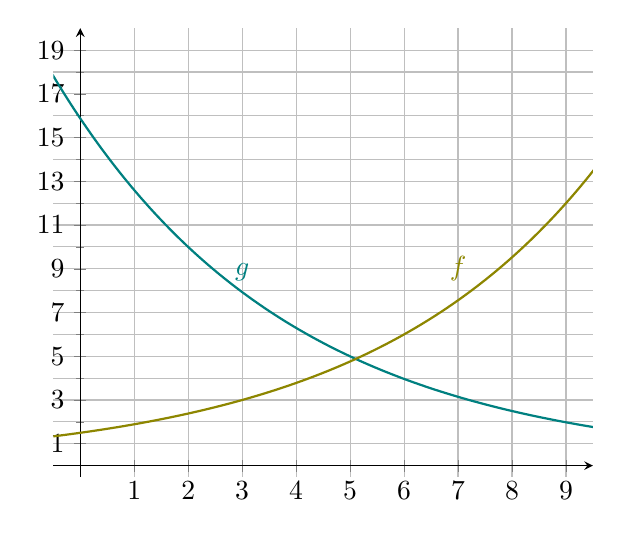
\begin{tikzpicture}
	\begin{axis}[
	axis lines = center, 
	xmin = -0.5, xmax = 9.5,
	ymin = -0.5, ymax = 20,
	grid = both,
	xtick = {-1,0,...,9,10},
	ytick = {-1,1,...,17,19},
	minor y tick num = 1
	]
		\addplot[thick, color = teal, domain = -1:10, samples = 200] {15.874*0.79370^x};
		\addplot[thick, color = olive, domain = -1:10, samples = 200] {1.5000*1.2599^x};
		\node[color = olive, anchor = south] at (axis cs: 7,8) {$f$};
		\node[color = teal, anchor = south] at (axis cs: 3,8) {$g$};
	\end{axis}
	\end{tikzpicture}
	\caption{Graferne for eksponentialfunktionerne $f$ og $g$.}
	\label{fig:forhalv}
\end{figure}
\begin{enumerate}[label=\roman*)]
	\item Bestem fordoblings-/halveringskonstanten for de to funktioner.
	\item Løs ligningen $f(x) = g(x)$. Afrund til nærmeste heltal.
\end{enumerate}

\subsection*{Opgave 9 (Uden hjælpemidler)}
På Figur \ref{fig:potens} ses graferne for tre potensfunktioner.
\begin{figure}[H]
	\centering
	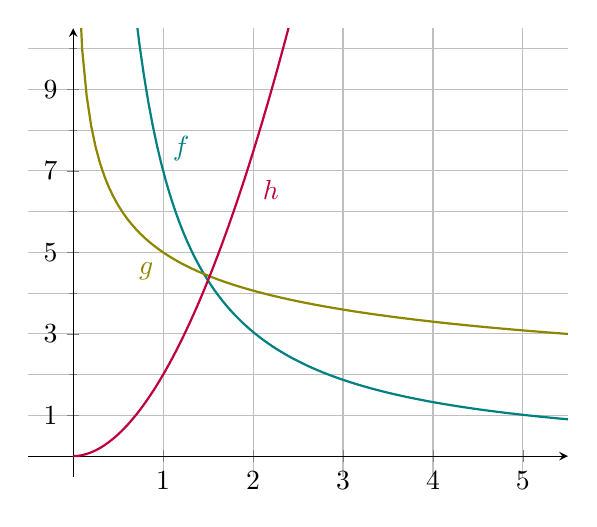
\begin{tikzpicture}
	\begin{axis}[
	axis lines = center, 
	xmin = -0.5, xmax = 5.5,
	ymin = -0.5, ymax = 10.5,
	grid = both,
	xtick = {-1,0,...,9,10},
	ytick = {-1,1,...,17,19},
	minor y tick num = 1
	]
		\addplot[thick, color = teal, domain = 0.5:10, samples = 200] {7*x^(-1.2)};
		\addplot[thick, color = olive, domain = 0.05:10, samples = 200] {5*x^(-0.3)};
		\addplot[thick, color = purple, domain = 0:10, samples = 200] {2*x^(1.9)};
		\node[color = teal, anchor = south west] at (axis cs: 1,7) {$f$};
		\node[color = olive, anchor = north east] at (axis cs: 1,5) {$g$};
		\node[color = purple, anchor = north west] at (axis cs: 2,7) {$h$};
	\end{axis}
	\end{tikzpicture}
	\caption{Graferne for potensfunktionerne $f$, $g$ og $h$.}
	\label{fig:potens}
\end{figure}
\begin{enumerate}[label=\roman*)]
	\item Bestem $b$-værdien for hver af de tre potensfunktioner $f$, $g$ og $h$. 
	\item Afgør, hvilke af de tre følgende intervaller, $a$-værdierne ligger i for de tre potensfunktioner. 
	\begin{align*}
		&a < 0,\\
		&1 > a > 0,\\
		&a > 1.
	\end{align*}
\end{enumerate}

\subsection*{Opgave 10 (Med hjælpemidler)}
Grafen for en potensfunktion $f$ skærer gennem punkterne $(2,9)$ og $(6,31)$. 
\begin{enumerate}[label=\roman*)]
	\item Bestem en forskrift for $f$. 
	\item Bestem tallet $f(9)$. 
	\item Løs ligningen $f(x) = 100$.
\end{enumerate}

\subsection*{Opgave 11 (Med hjælpemidler)}

En styrketræningsgruppe har henover en række måneder målt deres løfteevne på et bestemt løft. De har samlet deres data i \href{https://github.com/ChristianJLex/TeachingNotes/raw/master/2024-2025/Data og lign/Traening.xlsx}{\color{blue!60} dette datasæt.} De antager, at løfteevnen kan beskrives ved en sammenhæng $L$ givet ved 
\begin{align*}
	L(x) = b\cdot x^a,
\end{align*}
hvor $x$ betegner den forløbne tid i måneder og $L$ er løfteevnen i kg. 

\begin{enumerate}[label=\roman*)]
	\item Brug datasættet til at bestemme tallene $b$ og $a$. 
	\item Afgør, hvor længe de skal træne for at forvente at kunne løfte 100kg.
\end{enumerate}

\subsection*{Opgave 12 (Uden hjælpemidler)}

Et rektangel med bredde $5x$ og højde $2x$ er givet
\begin{enumerate}[label=\roman*)]
	\item Opstil en sammenhæng, der beskriver arealet af rektanglet som funktion af tallet $x$. 
	\item Afgør, hvor meget større arealet af rektanglet bliver, hvis $x$ ganges med 4. 
\end{enumerate}